
\section{Optimisations}
\label{opt}

We may want our machine to learn more complex problems, where the patterns to learn are more obscure. We could use the \gls{perceptron} \gls{model} and increase the complexity of the model, but this is not very effective as this will drastically increase the computation. Instead we want to find solutions and optimisations to certain types of data that cut down on the number of \gls{neuron}s we use. There are many ways we can optimise for certain types of inputs, but we will look specifically at an unsupervised model, spatial data, and sequential data.

\subsection{Auto-encoders}

Auto-encoders are unsupervised neural networks, as they do not require target data, however, they still have target data to meet. They encode
(compress) the input data into a latent \gls{vec}, $z$, and then decode the latent \gls{vec} into an output that should resemble the input.

\begin{figure}[h]
\setlength{\unitlength}{0.14in}
\centering
\begin{picture}(10, 6) 

\put(0, 0){\framebox(10, 6){}}

\put(4.6, 1.9){\framebox(0.8, 2.2){$z$}}

\mline{0.3}{0.3}{4.0}{1.3}
\mline{0.3}{5.7}{4.0}{-1.3}
\mline{0.3}{0.3}{0.0}{5.4}
\mline{4.3}{1.6}{0.0}{2.8}

\mline{5.7}{4.4}{4.0}{1.3}
\mline{5.7}{1.6}{4.0}{-1.3}
\mline{9.7}{0.3}{0.0}{5.4}
\mline{5.7}{1.6}{0.0}{2.8}

\end{picture}
\caption{Autoencoder block, AE}
\label{fig:aebox}
\end{figure}

\begin{figure}[h]
\setlength{\unitlength}{0.14in}
\centering
\begin{picture}(11,3) 

\put(0.0, 0.6){\framebox(2.2, 2.2){$X_i$}}

\put(4.4, 0.6){\framebox(2.2, 2.2){AE}}

\put(8.8, 0.6){\framebox(2.2, 2.2){$\tilde{X_i}$}}


\mline{2.3}{1.7}{2.0}{0.0}
\mline{6.7}{1.7}{2.0}{0.0}

\end{picture}
\caption{$\tilde{X_i}$ is the decoded output that resembles the input.}
\label{fig:ae}
\end{figure}

If you replace $X_i$ with a function of $X_i$, $f(X_i)$, you can train an inverse function as the auto-encoder.

They train an inverse function $f^{-1}$ from a given function $f$.

$$X=\{X_1,X_2,\cdots,X_I\}$$

There are some common functions that lead to useful outcomes.
Where $f(x) = x$, the auto-encoder acts like a compressor, making it an effective lossy compression
technique to reduce broadband.
Where $f(x)$ is a noise filter, the auto-encoder acts as a denoiser, making it faster to render fragment shaders as you do not have to calculate every pixel.


\begin{figure}[h]
\setlength{\unitlength}{0.14in}
\centering
\begin{picture}(15.4,3) 

\put(0.0, 0.6){\framebox(2.2, 2.2){$X_i$}}

\put(4.4, 0.6){\framebox(2.2, 2.2){$f$}}

\put(8.8, 0.6){\framebox(2.2, 2.2){AE}}

\put(13.2, 0.6){\framebox(2.2, 2.2){$\tilde{X_i}$}}

\mline{2.3}{1.7}{2.0}{0.0}
\mline{6.7}{1.7}{2.0}{0.0}
\mline{11.1}{1.7}{2.0}{0.0}

\end{picture}
\caption{Using a function, we can produce new inputs for our auto-encoder.}
\end{figure}


\begin{figure}[ht]
\setlength{\unitlength}{0.14in}
\centering
\begin{picture}(15.4,3) 

\put(0.0, 0.6){\framebox(2.2, 2.2){$X_i$}}

\put(4.4, 0.6){\framebox(2.2, 2.2){$f$}}

\put(8.8, 0.6){\framebox(2.2, 2.2){$f^{-1}$}}

\put(13.2, 0.6){\framebox(2.2, 2.2){$\tilde{X_i}$}}

\mline{2.3}{1.7}{2.0}{0.0}
\mline{6.7}{1.7}{2.0}{0.0}
\mline{11.1}{1.7}{2.0}{0.0}

\end{picture}
\caption{The auto-encoder then behaves as an inverse of the input function.}
\label{fig:aef}
\end{figure}
\newpage
\subsection{Convolutional Neural Networks}

A convolutional neural network uses a variety of methods to reduce the computation on spatial data, i.e. where the surroundings of the data are important. One method we can use are convolutions, which are \gls{layer}s that find patterns in context of the spatial data easier.\cite[p.~7]{cnn}

This means that the network
requires less \gls{neuron}s, which reduces the risk of overfitting and also saves computation.

\begin{figure}[h]
\setlength{\unitlength}{0.14in}
\centering
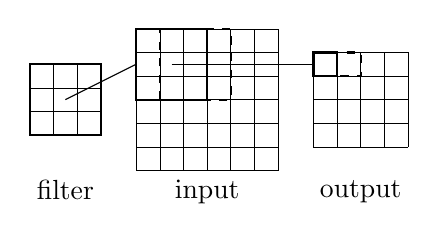
\begin{tikzpicture}[scale=0.30](18,3) 

\node at (1.5, 0) [below] {filter};
\node at (7.5, 0) [below] {input};
\node at (14, 0) [below] {output};

\draw[thick] (0,1.5) rectangle (3, 4.5);
\draw[thick] (12, 4) rectangle (13, 5);
\draw[thick, dashed] (13, 4) rectangle (14, 5);

\draw[thick] (4.5, 3) rectangle (7.5, 6);
\draw[thick, dashed] (5.5, 3) rectangle (8.5, 6);

\draw[step=1, very thin, yshift=0.5cm] (0, 1) grid (3, 4);
\draw[step=1, very thin, xshift=0.5cm] (4, 0) grid (10, 6);
\draw[step=1, very thin] (12, 1) grid (16, 5);

\draw (1.5, 3) -- (4.5, 4.5);
\draw (6, 4.5) -- (12, 4.5);

\end{tikzpicture}
\caption{Output is the convolution of the input given the filter.}
\label{fig:conv}
\end{figure}

The output from a convolution is a \gls{mat} where each node corresponds to the sum of encapsulated nodes multiplied by the filter's respective node.

\begin{equation}
\mx{O}_{ij}=\sum^{1}_{x=-1}{\sum^{1}_{y=-1}{\mx{I}_{(i+x+1)(j+y+1)}\times \mx{F}_{(x+1)(y+1)}}}
\end{equation}

or simply

\begin{equation}
\begin{split}
\mx{O}_{ij}&=\sum^{2}_{x=0}{\sum^{2}_{y=0}{\mx{I}_{(i+x)(j+y)}\times \mx{F}_{xy}}}\\
&=\sum^{X-1}_{x=0}{\sum^{Y-1}_{y=0}{\mx{I}_{(i+x)(j+y)}\times \mx{F}_{xy}}}
\end{split}
\end{equation}

To \gls{bprop} through convolutions, we will use a similar method to what we used in \sect{chain}.

\begin{equation}
\mx{O}=v(\mx{I},\mx{F})
\end{equation}

where $v$ is a function representing a convolution. 


Therefore we can decrease the \gls{cost} $C$, $\nabla C$, using the chain rule for the filter,

\begin{equation}
\begin{split}
\frac{\partial C}{\partial \mx{F}} &= \frac{\partial C}{\partial \mx{O}}\frac{\partial \mx{O}}{\partial \mx{F}}\\
\frac{\partial C}{\partial \mx{F}_{xy}} &= \sum_{i=0}^{I-1}{\sum_{j=0}^{J-1}{\frac{\partial C}{\partial \mx{O}_{ij}}\frac{\partial \mx{O}_{ij}}{\partial \mx{F}_{xy}}}}\\
&= \sum_{i=0}^{I-1}{\sum_{j=0}^{J-1}{\frac{\partial C}{\partial \mx{O}_{ij}}\mx{I-1}_{(i+x)(j+y)}}}\\
\frac{\partial C}{\partial \mx{F}} &=v(\mx{I}, \frac{\partial C}{\partial \mx{O}})
\end{split}
\end{equation}

and also for the image

\begin{equation}
\begin{split}
\frac{\partial C}{\partial \mx{I}} &= \frac{\partial C}{\partial \mx{O}}\frac{\partial \mx{O}}{\partial \mx{I}}\\
\frac{\partial C}{\partial \mx{I}_{ab}} &= \sum_{i=0}^{I-1}{\sum_{j=0}^{J-1}{\frac{\partial C}{\partial \mx{O}_{ij}}\frac{\partial \mx{O}_{ij}}{\partial \mx{I}_{ab}}}}\\
&= \sum_{x=0}^{X-1}{\sum_{y=0}^{Y-1}{\frac{\partial C}{\partial \mx{O}_{(a-x)(b-y)}}\mx{F}_{xy}}}\\
\frac{\partial C}{\partial \mx{I}} &= V(\frac{\partial C}{\partial \mx{O}}, R_{180\degree}\mx{F})
\end{split}
\end{equation}

where $V$ is a full convolution. A full convolution is a convolution that allows for a padding of the output, as $a-x$ or $b-y$ could be outside the range of output.\cite{backcnn}

\begin{figure}[h]
\setlength{\unitlength}{0.14in}
\centering
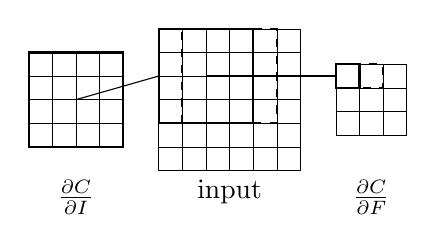
\begin{tikzpicture}[scale=0.30](18,3) 

\node at (2, 0) [below] {$\frac{\partial C}{\partial \mx{I}}$};
\node at (8.5, 0) [below] {input};
\node at (14.5, 0) [below] {$\frac{\partial C}{\partial \mx{F}}$};

\draw[thick] (0,1) rectangle (4, 5);
\draw[thick] (13, 3.5) rectangle (14, 4.5);
\draw[thick, dashed] (14, 3.5) rectangle (15, 4.5);

\draw[thick] (5.5, 2) rectangle (9.5, 6);
\draw[thick, dashed] (6.5, 2) rectangle (10.5, 6);

\draw[step=1, very thin, yshift=0.5cm] (13, 1) grid (16, 4);
\draw[step=1, very thin, xshift=0.5cm] (5, 0) grid (11, 6);
\draw[step=1, very thin] (0, 1) grid (4, 5);

\draw (2, 3) -- (5.5, 4);
\draw (7.5, 4) -- (13, 4);

\end{tikzpicture}
\caption{$\frac{\partial C}{\partial \mx{F}}$ is the output of a convolution with the filter $\frac{\partial C}{\partial \mx{I}}$ on the input.}
\label{fig:filterconv}
\end{figure}

\begin{figure}[h]
\setlength{\unitlength}{0.14in}
\centering
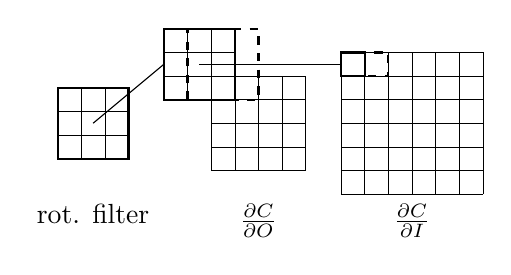
\begin{tikzpicture}[scale=0.30](18,3) 

\node at (1.5, 0) [below] {rot. filter};
\node at (15, 0) [below] {$\frac{\partial C}{\partial \mx{I}}$};
\node at (8.5, 0) [below] {$\frac{\partial C}{\partial \mx{O}}$};

\draw[thick] (0,1.5) rectangle (3, 4.5);
\draw[thick] (12, 5) rectangle (13, 6);
\draw[thick, dashed] (13, 5) rectangle (14, 6);

\draw[thick] (4.5, 4) rectangle (7.5, 7);
\draw[thick, dashed] (5.5, 4) rectangle (8.5, 7);

\draw[step=1, very thin, xshift=0.5cm] (4, 4) grid (7, 7);
\draw[step=1, very thin, yshift=0.5cm] (0, 1) grid (3, 4);
\draw[step=1, very thin] (12, 0) grid (18, 6);
\draw[step=1, very thin, xshift=0.5cm] (6, 1) grid (10, 5);

\draw (1.5, 3) -- (4.5, 5.5);
\draw (6, 5.5) -- (12, 5.5);

\end{tikzpicture}
\caption{$\frac{\partial C}{\partial \mx{I}}$ is the output of the full convolution $\frac{\partial C}{\partial \mx{O}}$ given a filter rotated by 180\degree}
\label{fig:fullconv}
\end{figure}

By using multiple convolutional \gls{layer}s in series, you teach the neural network to decompose features of the images, such as lines and shapes, which helps a feed-forward neural network to decrease the \gls{cost}. For example, the first \gls{layer} may pick out edges, the next lines, and then shapes.

We can also use pooling, which is a method of finding only the important information. It works similarly to a convolution, except the filter is constant, and uses a function instead of a summation, such as returning the maximum. This helps condense the output from convolutions.

In conclusion, we can use convolutions and pooling to help and optimise feed-forward networks to find patterns in spatial data. This is because the trainable parameters are only concerned in data surrounding a node. 

Moreover, this concludes that if we can differentiate a function to propagate forward and calculate a \gls{cost}, we are able to adjust the parameters of the function to decrease the \gls{cost}. 

\subsection{Recurrent Neural Networks}
\label{recurrent}

Recurrent neural networks are supervised neural networks that allow you to analyse sequential data. They work by feeding the current state into itself, which allows you to predict states of a system in the future based on the present.

\begin{figure}[ht]
\setlength{\unitlength}{0.14in}
\centering
\begin{picture}(10,7.2) 

\put(0.0, 0.6){\framebox(2.2, 2.2){$X$}}

\put(4.4, 0.6){\framebox(2.2, 2.2){$h$}}

\put(8.8, 0.6){\framebox(2.2, 2.2){$y$}}

\mline{2.3}{1.7}{2.0}{0.0}
\mline{6.7}{1.7}{2.0}{0.0}


\put(0.0, 5){\framebox(2.2, 2.2){$X$}}

\put(4.4, 5){\framebox(2.2, 2.2){$h$}}

\put(8.8, 5){\framebox(2.2, 2.2){$y$}}

\mline{2.3}{6.1}{2.0}{0.0}
\mline{6.7}{6.1}{2.0}{0.0}

\mline{5.4}{2.9}{0.0}{2.0}

\end{picture}
\caption{A recurrent neural network feeding the present state into the next.}
\label{fig:rnn}
\end{figure}

Back-propagating through this architecture is quite complex. It requires you to back-propagate through each state, which therefore implies that the more states you have, the more operations you would have to do. You would also have to store each of the inputs and outputs for each state.\cite{rnn}

Aside from this minor difference, the algebra of back-propagation is the same.